\documentclass[12pt,a4paper]{article}
%\usepackage{fontspec, xunicode, xltxtra}  
%\setmainfont{Hiragino Sans GB}  
\usepackage{xeCJK}
%\setCJKmainfont[BoldFont=STZhongsong, ItalicFont=STKaiti]{STSong}
%\setCJKsansfont[BoldFont=STHeiti]{STXihei}
%\setCJKmonofont{STFangsong}

%使用Xelatex编译

% 设置页面
%==================================================
\linespread{2} %行距
% \usepackage[top=1in,bottom=1in,left=1.25in,right=1.25in]{geometry}
% \headsep=2cm
% \textwidth=16cm \textheight=24.2cm
%==================================================

% 其它需要使用的宏包
%==================================================
\usepackage[colorlinks,linkcolor=blue,anchorcolor=red,citecolor=green,urlcolor=blue]{hyperref} 
\usepackage{tabularx}
\usepackage{authblk}         % 作者信息
\usepackage{algorithm}     % 算法排版
\usepackage{amsmath}     % 数学符号与公式
\usepackage{amsfonts}     % 数学符号与字体
\usepackage{mathrsfs}      % 花体
\usepackage{amssymb}
\usepackage[framemethod=TikZ]{mdframed}

\usepackage{graphicx} 
\usepackage{graphics}
\usepackage{color}
\usepackage{xcolor}
\usepackage{tcolorbox}
\usepackage{lipsum}
\usepackage{empheq}

\usepackage{fancyhdr}       % 设置页眉页脚
\usepackage{fancyvrb}       % 抄录环境
\usepackage{float}              % 管理浮动体
\usepackage{geometry}     % 定制页面格式
\usepackage{hyperref}       % 为PDF文档创建超链接
\usepackage{lineno}          % 生成行号
\usepackage{listings}        % 插入程序源代码
\usepackage{multicol}       % 多栏排版
%\usepackage{natbib}         % 管理文献引用
\usepackage{rotating}       % 旋转文字,图形,表格
\usepackage{subfigure}    % 排版子图形
\usepackage{titlesec}       % 改变章节标题格式
\usepackage{moresize}   % 更多字体大小
\usepackage{anysize}
\usepackage{indentfirst}  % 首段缩进
\usepackage{booktabs}   % 使用\multicolumn
\usepackage{multirow}    % 使用\multirow

\usepackage{wrapfig}
\usepackage{titlesec}     % 改变标题样式
\usepackage{enumitem}
\usepackage{aas_macros}

\newcommand{\myvec}[1]%
   {\stackrel{\raisebox{-2pt}[0pt][0pt]{\small$\rightharpoonup$}}{#1}}  %矢量符号
\renewcommand{\vec}[1]{\boldsymbol{#1}}
\newcommand{\me}{\mathrm{e}}
\newcommand{\mi}{\mathrm{i}}
\newcommand{\dif}{\mathrm{d}}
\newcommand{\tabincell}[2]{\begin{tabular}{@{}#1@{}}#2\end{tabular}}

\def\kpc{{\rm kpc}}
\def\km{{\rm km}}
\def\cm{{\rm cm}}
\def\TeV{{\rm TeV}}
\def\GeV{{\rm GeV}}
\def\MeV{{\rm MeV}}
\def\GV{{\rm GV}}
\def\MV{{\rm MV}}
\def\yr{{\rm yr}}
\def\s{{\rm s}}
\def\ns{{\rm ns}}
\def\GHz{{\rm GHz}}
\def\muGs{{\rm \mu Gs}}
\def\arcsec{{\rm arcsec}}
\def\K{{\rm K}}
\def\microK{\mu{\rm K}}
\def\sr{{\rm sr}}
\newcolumntype{p}{D{,}{\pm}{-1}}

\renewcommand{\figurename}{Fig.}
\renewcommand{\tablename}{Tab.}

\renewcommand{\arraystretch}{1.5}

\setlength{\parindent}{0pt}  %取消每段开头的空格

\title{Basic}
\author{}
\date{\today}
\begin{document}

\maketitle

\section{Preparation}

\subsection{初始设置}
对本地计算机里安装的Git进行设置

设置使用 Git 时的姓名和邮箱地址
\begin{tcolorbox}[colback=green!5,colframe=green!40!black,title= ]
$\$$ \textcolor{red}{git config $--$global user.name ``Firstname Lastname"} \\
$\$$ \textcolor{red}{git config $--$global user.email ``$\rm your\_email@example.com$"}
\end{tcolorbox}
这个命令,会在``$\rm \sim/.gitconfig$”中以如下形式输出设置文件
\begin{tcolorbox}[colback=green!5,colframe=green!40!black,title= ]
[user] \\
name = Firstname Lastname \\
email = $\rm your\_email@example.com$
\end{tcolorbox}
想更改这些信息时,可以直接编辑这个设置文件。这里设置的姓名和邮箱地址会用在 Git 的提交日志中。由于在 GitHub 上公开仓库时,这里的姓名和邮箱地址也会随着提交日志一同被公开,所以请不要使用不便公开的隐私信息。

将 color.ui 设置为 auto 可以让命令的输出拥有更高的可读性
\begin{tcolorbox}[colback=green!5,colframe=green!40!black,title= ]
$\$$ git config $--$global color.ui auto 
\end{tcolorbox}
``$\rm \sim/.gitconfig$”中会增加下面一行。
\begin{tcolorbox}[colback=green!5,colframe=green!40!black,title= ]
[color] \\
ui = auto
\end{tcolorbox}

\subsection{设置 SSH Key}
GitHub 上连接已有仓库时的认证,是通过使用了 SSH 的公开密钥认证方式进行的。创建公开密钥认证所需的 SSH Key,并将其添加至 GitHub。运行下面的命令创建 SSH Key
\begin{tcolorbox}[colback=green!5,colframe=green!40!black,title= ]
$\$$ \textcolor{red}{ssh-keygen -t rsa -C ``$\rm your\_email@example.com$"} \\
Generating public/private rsa key pair. \\
Enter file in which to save the key \\
$\rm (/Users/your\_user\_directory/.ssh/id\_rsa)$: 按回车键 \\
Enter passphrase (empty for no passphrase): 输入密码 \\
Enter same passphrase again: 再次输入密码
\end{tcolorbox}
``$\rm your\_email@example.com$”的部分请改成您在创建账户时用的邮箱地址。密码需要在认证时输入,请选择复杂度高并且容易记忆的组合。输入密码后会出现以下结果
\begin{tcolorbox}[colback=green!5,colframe=green!40!black,title= ]
Your identification has been saved in $\rm /Users/your\_user\_directory/.ssh/id\_rsa$. \\
Your public key has been saved in $\rm /Users/your\_user\_directory/.ssh/id\_rsa.pub$. \\
The key fingerprint is: \\
fingerprint值 $\rm your\_email@example.com$ \\
The key's randomart image is:
\end{tcolorbox}
$\rm id\_rsa$ 文件是私有密钥,$\rm id\_rsa.pub$ 是公开密钥。

在 GitHub 中添加公开密钥,今后就可以用私有密钥进行认证了。点击右上角的账户设定按钮( Account Settings),选择 SSH Keys 菜单。点击 Add SSH Key 之后,会出现输入框。在 Title 中输入适当的密钥名称。 Key 部分请粘贴 $\rm id\_rsa.pub$ 文件里的内容。 $\rm id\_rsa.pub$的内容可以用如下方法查看
\begin{tcolorbox}[colback=green!5,colframe=green!40!black,title= ]
$\$$ cat $\rm \sim/.ssh/id\_rsa.pub$ \\
ssh-rsa 公开密钥的内容 $\rm your\_email@example.com$
\end{tcolorbox}
添加成功之后,创建账户时所用的邮箱会接到一封提示“公共密钥添加完成”的邮件。完成以上设置后,就可以用手中的私人密钥与 GitHub 进行认证和通信了。
\begin{tcolorbox}[colback=green!5,colframe=green!40!black,title= ]
$\$$ ssh -T git@github.com \\
The authenticity of host 'github.com (207.97.227.239)' can't be established. \\
RSA key fingerprint is fingerprint值 . \\
Are you sure you want to continue connecting (yes/no)? 输入yes 
\end{tcolorbox}
出现如下结果即为成功 
\begin{tcolorbox}[colback=green!5,colframe=green!40!black,title= ]
Hi hirocastest! You've successfully authenticated, but GitHub does not provide shell access.
\end{tcolorbox}
创建一个公开的仓库。点击右上角工具栏里的 New repository 图标,创建新的仓库。

在 Initialize this repository with a README 选项上打钩,随后 GitHub 会自动初始化仓库并设置 README 文件,让用户可以立刻clone 这个仓库。如果想向 GitHub 添加手中已有的 Git 仓库,建议不要勾选,直接手动 push。

下方左侧的下拉菜单非常方便,通过它可以在\textcolor{yellow}{初始化时自动生成 .gitignore 文件\footnote{该文件用来描述 Git 仓库中不需管理的文件与目录。}}。这个设定会帮我们把\textcolor{yellow}{不需要在 Git 仓库中进行版本管理的文件记录在 .gitignore 文件中},省去了每次根据框架进行设置的麻烦。下拉菜单中包含了主要的语言及框架,选择今后将要使用的即可。

右侧的下拉菜单可以选择要添加的许可协议文件。如果这个仓库中包含的代码已经确定了许可协议,那么请在这里进行选择。随后将自动生成包含许可协议内容的 LICENSE 文件,用来表明该仓库内容的许可协议。

输入选择都完成后,点击 Create repository 按钮,完成仓库的创建。

下面这个 URL 便是刚刚创建的仓库的页面
\begin{tcolorbox}[colback=green!5,colframe=green!40!black,title= ]
https://github.com/用户名/Hello-Word
\end{tcolorbox}

README.md 在初始化时已经生成好了。README.md 文件的内容会自动显示在仓库的首页当中。因此,人们一般会在这个文件中标明本仓库所包含的软件的概要、使用流程、许可协议等信息。如果使用Markdown 语法进行描述,还可以添加标记,提高可读性。

在 GitHub 上进行交流时用到的 Issue、评论、 Wiki,都可以用Markdown 语法表述,从而进行标记。准确地说应该是 GitHub Flavored Markdown( GFM)语法。该语法虽然是 GitHub 在 Markdown 语法基础上扩充而来的,但一般情况下只要按照原本的 Markdown 语法进行描述就可以。使用 GitHub 后,很多文档都需要用 Markdown 来书写。

将已有仓库 clone 到身边的开发环境中。
\begin{tcolorbox}[colback=green!5,colframe=green!40!black,title= ]
$\$$ git clone git@github.com:hirocastest/Hello-World.git \\
Cloning into 'Hello-World'... \\
remote: Counting objects: 3, done. \\
remote: Total 3 (delta 0), reused 0 (delta 0) \\
Receiving objects: $100\% (3/3)$, done.
\end{tcolorbox}
这里会要求输入 GitHub 上设置的公开密钥的密码。认证成功后,仓库便会被 clone 至仓库名后的目录中。将想要公开的代码提交至这个仓库再 push 到 GitHub 的仓库中,代码便会被公开。

添加至 Git 仓库的文件显示为 Untracked files。通过 \textcolor{red}{git add} 命令将文件加入暂存区 A,再通过 \textcolor{red}{git commit} 命令提交。添加成功后,可以通过 \textcolor{red}{git log} 命令查看提交日志。之后只要执行 \textcolor{red}{git push},GitHub 上的仓库就会被更新。



\section{基本操作}
\cite{demaree2016git} Git commands :
\begin{tcolorbox}[colback=green!5,colframe=green!40!black,title= ]
\textcolor{blue}{(master) $\$:$ git commandname parameter1 parameter2 $--$option}
\end{tcolorbox}
The command name (commandname in the example) is one of over $100$ individual functions that Git can perform. Behind the scenes, each of these commands is a separate program responsible for its own specific job. 

Options are special parameters that are denoted by at least one leading dash character. Many options have both a \textcolor{orange}{long form}, like \textcolor{blue}{$--$global}, and a \textcolor{orange}{shortcut form}, like \textcolor{blue}{$-$g}. There are also options that take values, like \textcolor{blue}{git commit $--$message=``hello world"}.

There are two that it absolutely needs in order to function: \textcolor{red}{your name} and \textcolor{red}{email address}. \textcolor{orange}{Git adds an Author attribute to every commit you make} that includes both your name and email address, so that your collaborators on a project can know who made a given change. The name you enter will be used to identify you in change logs and any other place where Git shows who made a particular change, while your email address
not only tells people how to reach you, but also tells a hosted service like GitHub who you are on their service.

Use the \textcolor{blue}{git config} command to tell Git who you are. Unlike most Git commands, which \textcolor{orange}{only work inside of a Git project}, these can be \textcolor{orange}{run from any directory}. 

要使用 Git 进行版本管理,必须先初始化仓库。 Git 是使用 \textcolor{red}{\bf git init} 命令\textcolor{blue}{进行初始化}的。建立一个目录并初始化仓库。如果初始化成功,执行了 git init命令的目录下就会生成 \textcolor{red}{.git 目录}。这个 .git 目录里\textcolor{blue}{存储着管理当前目录内容所需的仓库数据}。

在 Git 中,将这个目录的内容称为``\textcolor{blue}{附属于该仓库的工作树}”。文件的编辑等操作在工作树中进行,然后记录到仓库中,以此管理文件的历史快照。如果想将文件恢复到原先的状态,可以从仓库中调取之前的快照,在工作树中打开。开发者可以通过这种方式获取以往的文件。

 \textcolor{red}{\bf git status} 命令用于显示 Git 仓库的状态。工作树和仓库在被操作的过程中,状态会不断发生变化。在 Git 操
作过程中时常用 git status 命令查看当前状态。
\begin{tcolorbox}[colback=green!5,colframe=green!40!black,title= ]
$\$$ git status \\
$\#$ On branch master \\
$\#$  \\
$\#$  Initial commit \\
$\#$  \\
nothing to commit (create/copy files and use ``git add" to track) 
\end{tcolorbox}
结果显示了当前正处于 master 分支下。接着还显示了没有可提交的内容。所谓\textcolor{red}{提交(Commit)},是指``\textcolor{orange}{记录工作树中所有文件的当前状态}"。尚没有可提交的内容,就是说当前建立的这个仓库中还没有记录任何文件的任何状态。只要对 Git 的工作树或仓库进行操作, git status 命令的显示结果就会发生变化。

如果只是用 Git 仓库的工作树创建了文件,那么该文件并不会被记入 Git 仓库的版本管理对象当中。要想让文件成为 Git 仓库的管理对象,就需要用 \textcolor{red}{\bf git add} 命令将其\textcolor{orange}{加入暂存区}(Stage 或者 Index)中。\textcolor{blue}{暂存区是提交之前的一个临时区域}。
\begin{tcolorbox}[colback=green!5,colframe=green!40!black,title= ]
$\$$ git add README.md \\
$\$$ git status \\
$\#$ On branch master \\
$\#$ \\
$\#$ Initial commit \\
$\#$ \\
$\#$ Changes to be committed: \\
$\#$ (use ``git rm $--$cached <file>..." to unstage) \\
$\#$ \\
$\#$ new file: README.md 
\end{tcolorbox}
README.md 文件显示在 Changes to be committed 中了。

\textcolor{red}{\bf git commit }命令可以\textcolor{blue}{将当前暂存区中的文件实际保存到仓库的历史记录中。通过这些记录,可以在工作树中复原文件。}
\begin{tcolorbox}[colback=green!5,colframe=green!40!black,title= ]
$\$$ git commit $\rm -m$ ``First commit" \\
$\rm [master (root-commit) 9f129ba]$ First commit \\
1 file changed, 0 insertions(+), 0 deletions(-) \\
create mode 100644 README.md 
\end{tcolorbox}
\textcolor{orange}{-m 参数后}的 ``First commit"称作\textcolor{red}{提交信息},\textcolor{orange}{是对这个提交的概述}。想要记述得更加详细,\textcolor{orange}{不加 -m},\textcolor{red}{直接执行 git commit命令}。执行后编辑器就会启动,并显示如下结果
\begin{tcolorbox}[colback=green!5,colframe=green!40!black,title= ]
$\#$ Please enter the commit message for your changes. Lines starting \\
$\#$ with '$\#$' will be ignored, and an empty message aborts the commit. \\
$\#$ On branch master \\
$\#$ \\
$\#$ Initial commit \\
$\#$ \\
$\#$ Changes to be committed: \\
$\#$ (use ``git rm $--$cached <file>..." to unstage) \\
$\#$ \\
$\#$ new file: README.md 
\end{tcolorbox}
在编辑器中\textcolor{orange}{记述提交信息的格式}如下: \\
第一行:用一行文字简述提交的更改内容 \\
第二行:空行 \\
第三行以后:记述更改的原因和详细内容 

只要按照上面的格式输入,今后可以通过确认日志的命令或工具看到这些记录。在\textcolor{orange}{以 $\#$(井号)标为注释的 Changes to be committed(要提交的更改)栏中,可以查看本次提交中包含的文件}。将提交信息按格式记述完毕后,请保存并关闭编辑器,以$\#$(井号)标为注释的行不必删除。随后,刚才记述的提交信息就会被提交。

如果在编辑器启动后想中止提交,请将提交信息留空并直接关闭编辑器,随后提交就会被中止。

当前工作树处于刚刚完成提交的最新状态,所以结果显示没有更改。

\textcolor{red}{\bf git log} 命令可以\textcolor{blue}{查看以往仓库中提交的日志}。包括可以查看什么人在什么时候进行了提交或合并,以及操作前后有怎样的差别。
\begin{tcolorbox}[colback=green!5,colframe=green!40!black,title= ]
$\$$ git log \\
commit 9f129bae19b2c82fb4e98cde5890e52a6c546922 \\
Author: hirocaster <hohtsuka@gmail.com> \\
Date: Sun May 5 16:06:49 2013 +0900 \\
First commit 
\end{tcolorbox}
commit 栏旁边显示的``9f129b……"是\textcolor{blue}{指向这个提交的哈希值}。 Git 的其他命令中,在指向提交时会用到这个哈希值。Author 栏中显示 Git 设置的用户名和邮箱地址。 Date 栏中显示提交执行的日期和时间。再往下就是该提交的提交信息。

如果只想让程序显示第一行简述信息,可以在 git log命令后加上 \textcolor{violet}{$--$pretty=short}。
\begin{tcolorbox}[colback=green!5,colframe=green!40!black,title= ]
$\$$ git log --pretty=short \\
commit 9f129bae19b2c82fb4e98cde5890e52a6c546922 \\
Author: hirocaster <hohtsuka@gmail.com> \\
First commit
\end{tcolorbox}
只要在 \textcolor{blue}{git log 命令后加上目录名},便会\textcolor{blue}{只显示该目录下的日志}。如果\textcolor{blue}{加的是文件名},就会\textcolor{blue}{只显示与该文件相关的日志}。
\begin{tcolorbox}[colback=green!5,colframe=green!40!black,title= ]
$\$$ git log README.md
\end{tcolorbox}

如果想\textcolor{blue}{查看提交所带来的改动},可以加上 \textcolor{red}{\bf -p} 参数,\textcolor{blue}{文件的前后差别就会显示在提交信息之后}。
\begin{tcolorbox}[colback=green!5,colframe=green!40!black,title= ]
$\$$ git log -p
\end{tcolorbox}

只查看 README.md 文件的提交日志以及提交前后的差别
\begin{tcolorbox}[colback=green!5,colframe=green!40!black,title= ]
$\$$ git log -p README.md
\end{tcolorbox}
\textcolor{red}{\bf git diff} 命令可以\textcolor{blue}{查看工作树、暂存区、最新提交之间的差别}。如果尚未用 git add命令向暂存区添加任何东西,所以程序只会显示工作树与最新提交状态之间的差别。\textcolor{red}{``+”号}标出的是\textcolor{blue}{新添加的行},\textcolor{blue}{被删除的行}则用\textcolor{red}{``-”号}标出。可以看到,这次只添加了一行。
\begin{tcolorbox}[colback=green!5,colframe=green!40!black,title= ]
$\$$ git diff \\
diff $--$git a/README.md b/README.md \\
index e69de29..cb5dc9f 100644 \\
$---$ a/README.md \\
+++ b/README.md \\
@@ -0,0 +1 @@ \\
+$\#$ Git教程
\end{tcolorbox}
如果现在执行 git diff 命令,由于工作树和暂存区的状态并无差别,结果什么都不会显示。要查看与最新提交的差别,执行以下命令
\begin{tcolorbox}[colback=green!5,colframe=green!40!black,title= ]
$\$$ git diff HEAD \\
diff $--$git a/README.md b/README.md \\
index e69de29..cb5dc9f 100644 \\
$---$ a/README.md \\
+++ b/README.md \\
@@ -0,0 +1 @@ \\
+$\#$ Git教程
\end{tcolorbox}
\textcolor{violet}{在执行 git commit 命令之前先执行git diff HEAD命令,查看本次提交与上次提交之间有什么差别,等确认完毕后再进行提交}。这里的 \textcolor{blue}{HEAD 是指向当前分支中最新一次提交的指针}。


\cite{narębski2016mastering} If you want to know not only which files were changed (which you get with git status), but also what exactly you have changed, use the \textcolor{red}{\bf git diff} command. In Git there are \textcolor{orange}{three stages}: the \textcolor{red}{working directory}, the \textcolor{orange}{staging area}, and the \textcolor{orange}{repository} (usually the last commit). Therefore, we have not one set of differences but three, as shown in Fig \ref{FIG:git_diff}.

\begin{figure}
\begin{center}
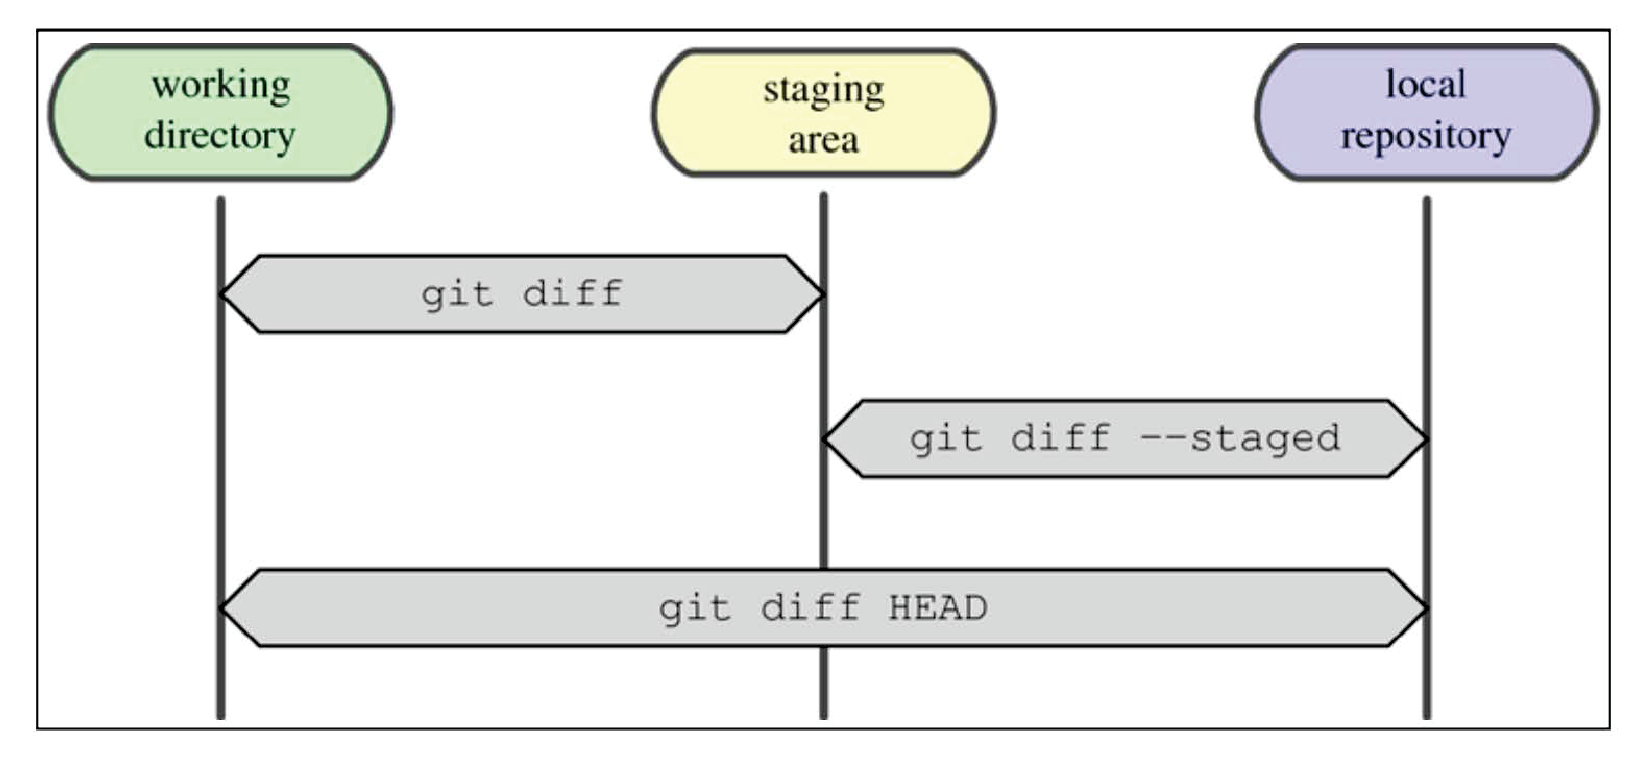
\includegraphics[width=12cm]{git_diff.eps}
\caption{Examining the differences between the working directory, staging area, and local git repository. 
}
\label{FIG:git_diff}
\end{center}
\end{figure}

To see \textcolor{blue}{what you've changed but not yet staged}, type \textcolor{blue}{git diff} with no other arguments. This command compares what is in your \textcolor{blue}{working directory} with what is in your \textcolor{blue}{staging area}. These are the changes that could be added, but wouldn't be present if we create commit with \textcolor{blue}{git commit} (without \textcolor{blue}{-a}): \textit{Changes not staged for commit} in the \textcolor{blue}{git status} output. 

To see \textcolor{blue}{what you've staged that will go into your next commit}, use \textcolor{blue}{git diff $--$staged} (or \textcolor{blue}{git diff $--$cached}). This command compares what is in your staging area to the content of your last commit. These are the changes that would be added with git commit (without -a): Changes to be committed in the git status output. You can \textcolor{blue}{compare your staging area to any commit} with \textcolor{red}{git diff $--$staged <commit>}; HEAD (the last commit) is just the default.

You can use \textcolor{red}{git diff HEAD} to \textcolor{blue}{compare what is in your working directory with the last commit} (or arbitrary commit with \textcolor{red}{git diff <commit>}). These are the changes that would be added with the git commit -a shortcut.

If you are using \textcolor{red}{git commit -a}, and not making use of the staging area, usually it is enough to use git diff to check the changes which will be in the next commit. The only issue is the \textcolor{yellow}{new files that are added with bare \textit{git add} }; they \textcolor{yellow}{won't show in the git diff output} unless you use \textcolor{red}{git add $--$intent-to-add} (or its equivalent \textcolor{red}{git add -N}) to add new files.



\section{分支的操作}
在进行多个并行作业时,会用到分支。在这类并行开发的过程中,往往同时存在多个最新代码状态。从 master 分支创
建 feature-A 分支和 fix-B 分支后,每个分支中都拥有自己的最新代码。master 分支是 Git 默认创建的分支,因此基本上所有开发都是以这个分支为中心进行的。不同分支中,可以同时进行完全不同的作业。等该分支的作业完成之后再与 master 分支合并。比如 feature-A 分支的作业结束后与 master 合并。

\textcolor{red}{\bf git branch} 命令可以\textcolor{blue}{将分支名列表显示},同时可以 \textcolor{blue}{确认当前所在分支}。
\begin{tcolorbox}[colback=green!5,colframe=green!40!black,title= ]
$\$$ git branch \\
$\ast$ master
\end{tcolorbox}
master 分支左侧标有``$\ast$"(星号),表示当前所在的分支。也就是说,正在 master 分支下进行开发。结果中没有显示其他分支名,表示本地仓库中只存在 master 一个分支。

如果想以当前的 master 分支为基础创建新的分支,需要用到 \textcolor{red}{\bf git checkout -b} 命令。创建名为 feature-A 的分支
\begin{tcolorbox}[colback=green!5,colframe=green!40!black,title= ]
$\$$ git checkout -b feature-A \\
Switched to a new branch `feature-A'
\end{tcolorbox}
连续执行下面两条命令也能收到同样效果
\begin{tcolorbox}[colback=green!5,colframe=green!40!black,title= ]
$\$$ \textcolor{green}{git branch feature-A} \\
$\$$ \textcolor{green}{git checkout feature-A}
\end{tcolorbox}
创建 feature-A 分支,并将当前分支切换为 feature-A 分支。这时查看分支列表,会显示处于 feature-A 分支下。
\begin{tcolorbox}[colback=green!5,colframe=green!40!black,title= ]
$\$$ git branch \\
$\ast$ feature-A \\
master 
\end{tcolorbox}
feature-A 分支左侧标有``$\ast$”,表示当前分支为 feature-A。在这个状态下像正常开发那样修改代码、执行 git add命令并进行提交的话,代码就会提交至 feature-A 分支。 像这样 \textcolor{blue}{不断对一个分支(例如feature-A)进行提交的操作},称为`` \textcolor{red}{培育分支}”。

切换至master 分支
\begin{tcolorbox}[colback=green!5,colframe=green!40!black,title= ]
$\$$ git checkout master \\
Switched to branch `master'
\end{tcolorbox}
查看 README.md 文件,会发现 README.md 文件仍然保持原先的状态,并没有被添加文字。 feature-A 分支的更改不会影响到 master 分支,这正是在开发中创建分支的优点。只要创建多个分支,就可以在不互相影响的情况下同时进行多个功能的开发。
\begin{tcolorbox}[colback=green!5,colframe=green!40!black,title= ]
$\$$ \textcolor{green}{git checkout $-$} \\
Switched to branch `feature-A'
\end{tcolorbox}
用\textcolor{red}{``$-$"(连字符)代替分支名},就可以切换至上一个分支。当然,将``$-$"替换成 feature-A 同样可以切换到 feature-A 分支。

\textcolor{red}{特性分支},是集中实现单一特性(主题),除此之外不进行任何作业的分支。在日常开发中,往往会创建数个特性分支,同时在此之外再保留一个随时可以发布软件的稳定分支。稳定分支的角色通常由 master 分支担当。

之前创建了 feature-A 分支,这一分支主要实现 feature-A,除 feature-A 的实现之外不进行任何作业。即便在开发过程中发现了 BUG,也需要再创建新的分支,在新分支中进行修正。基于特定主题的作业在特性分支中进行,主题完成后再与 master 分支合并。只要保持这样一个开发流程,就能保证 master 分支可以随时供人查看。这样一来,其他开发者也可以放心大胆地从 master 分支创建新的特性分支。


主干分支是特性分支的原点,同时也是合并的终点。通常人们会用 master 分支作为主干分支。主干分支中并没有开发到一半的代码,可以随时供他人查看。

假设 feature-A 已经实现完毕,想要将它合并到主干分支 master 中。首先切换到 master 分支
\begin{tcolorbox}[colback=green!5,colframe=green!40!black,title= ]
$\$$ git checkout master \\
Switched to branch `master'
\end{tcolorbox}
然后合并 feature-A 分支。为了在历史记录中明确记录下本次分支合并,需要创建合并提交。因此,在合并时加上 \textcolor{red}{\bf $--$no-ff} 参数。
\begin{tcolorbox}[colback=green!5,colframe=green!40!black,title= ]
$\$$ git merge $--$no-ff feature-A
\end{tcolorbox}
随后编辑器会启动,用于录入合并提交的信息
\begin{tcolorbox}[colback=green!5,colframe=green!40!black,title= ]
Merge branch `feature-A' \\
$\#$ Please enter a commit message to explain why this merge is necessary, especially if it merges an updated upstream into a topic branch. \\
$\#$ \\
$\#$ Lines starting with `$\#$' will be ignored, and an empty message aborts the commit.
\end{tcolorbox}
默认信息中已经包含了是从 feature-A 分支合并过来的相关内容,所以可不必做任何更改。将编辑器中显示的内容保存,关闭编辑器,然后就会看到
\begin{tcolorbox}[colback=green!5,colframe=green!40!black,title= ]
Merge made by the `recursive' strategy. \\
README.md | 2 ++ \\
1 file changed, 2 insertions(+)
\end{tcolorbox}
用 \textcolor{red}{git log $--$graph} 命令进行查看的话,能很清楚地看到特性分支(feature-A)提交的内容已被合并。除此以外,特性分支的创建以及合并也都清楚明了。
\begin{tcolorbox}[colback=green!5,colframe=green!40!black,title= ]
$\$$ git log $--$graph \\
$\ast$ commit 83b0b94268675cb715ac6c8a5bc1965938c15f62 \\
|\ Merge: fd0cbf0 8a6c8b9 \\
| | Author: hirocaster <hohtsuka@gmail.com> \\
| | Date: Sun May 5 16:37:57 2013 +0900 \\
| | \\
| | Merge branch `feature-A' \\
| | \\
| $\ast$ commit 8a6c8b97c8962cd44afb69c65f26d6e1a6c088d8 \\
|/ Author: hirocaster <hohtsuka@gmail.com> \\
| Date: Sun May 5 16:22:02 2013 +0900 \\
| \\
| Add feature-A \\
| \\
$\ast$ commit fd0cbf0d4a25f747230694d95cac1be72d33441d \\
| Author: hirocaster <hohtsuka@gmail.com> \\
| Date: Sun May 5 16:10:15 2013 +0900 \\
| \\
| Add index \\
| \\
$\ast$ commit 9f129bae19b2c82fb4e98cde5890e52a6c546922 \\
Author: hirocaster <hohtsuka@gmail.com> \\
Date: Sun May 5 16:06:49 2013 +0900 \\
First commit 
\end{tcolorbox}
git log $--$graph 命令可以用图表形式输出提交日志。

回溯历史版本,创建一个名为 fix-B 的特性分支。要让仓库的 HEAD、暂存区、当前工作树回溯到指定状态,需要用到 \textcolor{red}{\bf git rest --hard} 命令。只要提供目标时间点的哈希值\footnote{哈希值在每个环境中各不相同,需查看当前环境中 Add index 的哈希值,进行替换。},就可以完全恢复至该时间点的状态。
\begin{tcolorbox}[colback=green!5,colframe=green!40!black,title= ]
$\$$ git reset $--$hard fd0cbf0d4a25f747230694d95cac1be72d33441d \\
HEAD is now at fd0cbf0 Add index
\end{tcolorbox}
回溯到特性分支(feature-A)创建之前的状态。由于所有文件都回溯到了指定哈希值对应的时间点上, README.md 文件的内容也恢复到了当时的状态。
\begin{tcolorbox}[colback=green!5,colframe=green!40!black,title= ]
$\$$ git checkout -b fix-B \\
Switched to a new branch `fix-B'
\end{tcolorbox}
恢复到 feature-A 分支合并后的状态。不妨称这一操作为“推进历史”。

git log 命令只能查看以当前状态为终点的历史日志。所以这里要使用 \textcolor{red}{\bf git reflog} 命令,\textcolor{blue}{查看当前仓库的操作日志}。在日志中找出回溯历史之前的哈希值,通过 \textcolor{red}{\bf git reset --hard} 命令恢复到回溯历史前的状态。

执行 git reflog 命令,查看当前仓库执行过的操作的日志。
\begin{tcolorbox}[colback=green!5,colframe=green!40!black,title= ]
$\$$ git reflog \\
4096d9e HEAD@$\{0\}$: commit: Fix B \\
fd0cbf0 HEAD@$\{1\}$: checkout: moving from master to fix-B \\
fd0cbf0 HEAD@$\{2\}$: reset: moving to fd0cbf0d4a25f747230694d95cac1be72d33441d \\
83b0b94 HEAD@$\{3\}$: merge feature-A: Merge made by the 'recursive' strategy. \\
fd0cbf0 HEAD@$\{4\}$: checkout: moving from feature-A to master \\
8a6c8b9 HEAD@$\{5\}$: checkout: moving from master to feature-A \\
fd0cbf0 HEAD@$\{6\}$: checkout: moving from feature-A to master \\
8a6c8b9 HEAD@$\{7\}$: commit: Add feature-A \\
fd0cbf0 HEAD@$\{8\}$: checkout: moving from master to feature-A \\
fd0cbf0 HEAD@$\{9\}$: commit: Add index \\
9f129ba HEAD@$\{10\}$
\end{tcolorbox}

在日志中,可以看到 commit、 checkout、 reset、 merge 等 Git 命令的执行记录。只要不进行 Git 的 GC(Garbage Collection,垃圾回收),就可以通过日志随意调取近期的历史状态,就像给时间机器指定一个时间点,在过去未来中自由穿梭一般。即便开发者错误执行了 Git 操作,基本也都可以利用 git reflog命令恢复到原先的状态。


要修改上一条提交信息,可以使用 \textcolor{red}{\bf git commit $--$amend} 命令。


\section{推送至远程仓库}
为防止与其他仓库混淆,仓库名与本地仓库保持一致。创建时不要勾选 Initialize this repository with a README 选项。因为一旦勾选该选项, GitHub 一侧的仓库就会自动生成 README 文件,从创建之初便与本地仓库失去了整合性。虽然到时也可以强制覆盖,但为防止这一情况发生还是建议不要勾选该选项,直接点击 Create repository 创建仓库。

在 GitHub 上创建的仓库路径为``git@github.com:用户名/git-tutorial.git"。现在我们用 \textcolor{red}{\bf git remote add} 命令将它设置成本地仓库的远程仓库 A。
\begin{tcolorbox}[colback=green!5,colframe=green!40!black,title= ]
$\$$ git remote add origin git@github.com:github-book/git-tutorial.git
\end{tcolorbox}
按照上述格式执行 git remote add 命令之后,\textcolor{orange}{Git 会自动将 git@github.com:github-book/git-tutorial.git 远程仓库的名称}设置为 \textcolor{yellow}{origin(标识符)}。

\cite{narębski2016mastering} To add a new remote Git repository and to store its information under a shortname, run \textcolor{red}{\bf git remote add <shortname> <URL>}:
\begin{tcolorbox}[colback=green!5,colframe=green!40!black,title= ]
$\$$ git remote add alice https://git.company.com/alice/random.git
\end{tcolorbox}
Adding remote doesn't fetch from it automatically -- you need to use the \textcolor{red}{\bf -f} option for that (or run \textcolor{red}{\bf git fetch <shortname>}).

将当前分支下本地仓库中的内容推送给远程仓库,需要用到 \textcolor{red}{\bf git push} 命令。假定在 master 分支下进行操作
\begin{tcolorbox}[colback=green!5,colframe=green!40!black,title= ]
$\$$ git push -u origin master \\
Counting objects: $20$, done. \\
Delta compression using up to 8 threads. \\
Compressing objects: $100\%$ ($10/10$), done. \\
Writing objects: $100\%$ ($20/20$), 1.60 KiB, done. \\
Total $20$ (delta $3$), reused $0$ (delta $0$) \\
To git@github.com:github-book/git-tutorial.git \\
$\ast$ [new branch] master -> master \\
Branch master set up to track remote branch master from origin.
\end{tcolorbox}
像这样执行 git push命令,当前分支的内容就会被推送给远程仓库 origin 的 master 分支。\textcolor{red}{\bf -u}参数可以在推送的同时,\textcolor{yellow}{将 origin 仓库的 master 分支设置为本地仓库当前分支的 upstream(上游)。添加了这个参数,将来运行 git pull命令从远程仓库获取内容时,本地仓库的这个分支就可以直接从 origin 的 master 分支获取内容,省去了另外添加参数的麻烦。}

执行该操作后,当前本地仓库 master 分支的内容将会被推送到GitHub 的远程仓库中。在 GitHub 上也可以确认远程 master 分支的内容和本地 master 分支相同。

除了 master 分支之外,远程仓库也可以创建其他分支。在本地仓库中创建 feature-D 分支,并将它以同名形式 push 至远程仓库。
\begin{tcolorbox}[colback=green!5,colframe=green!40!black,title= ]
$\$$ git checkout -b feature-D \\
Switched to a new branch `feature-D'
\end{tcolorbox}
\begin{tcolorbox}[colback=green!5,colframe=green!40!black,title= ]
$\$$ git push -u origin feature-D \\
Total 0 (delta 0), reused 0 (delta 0) \\
To git@github.com:github-book/git-tutorial.git \\
$\ast$ [new branch] feature-D -> feature-D \\
Branch feature-D set up to track remote branch feature-D from origin.
\end{tcolorbox}



\cite{narębski2016mastering} While importing a subproject, you would want to be able to update the embedded files easily. You would want to continue interacting with the subproject. For this, you would add that subproject (for example, the common library) as a remote reference in your own (super) project and fetch it:
\begin{tcolorbox}[colback=green!5,colframe=green!40!black,title= ]
$\$$ git remote add mylib$\_$repo https://git.example.com/mylib.git \\
$\$$ git fetch mylib$\_$repo \\
warning: no common commits \\
remote: Counting objects: 12, done. \\
remote: Total 12 (delta 0), reused 0 (delta 0) \\
Unpacking objects: $100\%$ ($12/12$), done. \\
From https://git.example.com/mylib.git \\
$\ast$ [new branch] master -> mylib$\_$repo/master \\
\end{tcolorbox}

To see which remote repositories you have configured, you can run the \textcolor{red}{\bf git remote} command. It lists the shortnames of each remote you've got. In a cloned repository you will have at least one remote: origin.
\begin{tcolorbox}[colback=green!5,colframe=green!40!black,title= ]
$\$$ git remote \\
origin
\end{tcolorbox}

To see the URL together with remotes, you can use \textcolor{red}{\bf $-$v / $--$verbose} option
\begin{tcolorbox}[colback=green!5,colframe=green!40!black,title= ]
$\$$ git remote $--$verbose \\
origin git://git.kernel.org/pub/scm/git/git.git (fetch) \\
origin git://git.kernel.org/pub/scm/git/git.git (push)
\end{tcolorbox}

If you want to inspect remotes to see more information about a particular remote, use the \textcolor{red}{\bf git remote show <remote>} subcommand
\begin{tcolorbox}[colback=green!5,colframe=green!40!black,title= ]
$\$$ git remote show origin \\
$\ast$ remote origin \\
Fetch URL: git://git.kernel.org/pub/scm/git/git.git \\
Push URL: git://git.kernel.org/pub/scm/git/git.git \\
HEAD branch: master \\
Remote branches: \\
maint tracked \\
master tracked \\
next tracked \\
pu tracked \\
todo tracked \\
Local branch configured for `git pull': \\
master merges with remote master \\
Local ref configured for `git push': \\
master pushes to master (up-to-date)
\end{tcolorbox}

Git will consult the remote configuration, the branch configuration, and the remote repository (for an up-to-date status). If you want to skip contacting the remote repository and use cached information instead, add the \textcolor{red}{\bf $-$n} option to \textcolor{red}{\bf git remote show}.




In the centralized workflow, the integration is distributed: each developer is responsible for merging changes (in their topic branches), and publishing the result to the master branch in the central repository. You would need to update the local master branch, merge the topic branch to it, and push it:
\begin{tcolorbox}[colback=green!5,colframe=green!40!black,title= ]
$\$$ git checkout master \\
$\$$ git pull \\
$\$$ git merge feature-foo \\
$\$$ git push origin master
\end{tcolorbox}


\section{从远程仓库获取}
将 GitHub 上的仓库 clone 到本地。
\begin{tcolorbox}[colback=green!5,colframe=green!40!black,title= ]
$\$$ git clone git@github.com:github-book/git-tutorial.git \\
Cloning into `git-tutorial'... \\
remote: Counting objects: $20$, done. \\
remote: Compressing objects: $100\%$ ($7/7$), done. \\
remote: Total $20$ (delta $3$), reused $20$ (delta $3$) \\
Receiving objects: $100\%$ ($20/20$), done. \\
Resolving deltas: $100\%$ ($3/3$), done. \\
\end{tcolorbox}
\textcolor{orange}{执行 git clone命令后会默认处于 master 分支下,同时系统会自动将 origin 设置成该远程仓库的标识符}。也就是说,\textcolor{orange}{当前本地仓库的 master 分支与 GitHub 端远程仓库(origin)的 master 分支在内容上是完全相同的}。
\begin{tcolorbox}[colback=green!5,colframe=green!40!black,title= ]
$\$$ git branch -a \\
$\ast$ master \\
remotes/origin/HEAD -> origin/master \\
remotes/origin/feature-D \\
remotes/origin/master 
\end{tcolorbox}
用 \textcolor{red}{\bf git branch -a} 命令查看当前分支的相关信息。添加 \textcolor{red}{\bf -a} 参数可以同时显示本地仓库和远程仓库的分支信息。结果中显示了 remotes/origin/feature-D,证明远程仓库中已经有了 feature-D 分支。

将 feature-D 分支获取至本地仓库:
\begin{tcolorbox}[colback=green!5,colframe=green!40!black,title= ]
$\$$ git checkout -b feature-D origin/feature-D \\
Branch feature-D set up to track remote branch feature-D from origin. \\
Switched to a new branch `feature-D'
\end{tcolorbox}
 \textcolor{red}{\bf -b} 参数的后面是\textcolor{orange}{本地仓库中新建分支的名称}。新建分支名称后面是获取来源的分支名称。例子中指定了 origin/feature-D,就是说以名为 origin 的仓库(这里指 GitHub 端的仓库)的 feature-D 分支为来源,在本地仓库中创建 feature-D 分支。

假定是另一名开发者,要做一个新的提交。在 README.md 文件中添加一行文字,查看更改。
\begin{tcolorbox}[colback=green!5,colframe=green!40!black,title= ]
$\$$ git diff \\
diff $--$git a/README.md b/README.md \\
index af647fd..30378c9 100644 \\
$---$ a/README.md \\
+++ b/README.md \\
@@ $-3,3 +3,4$ @@ \\
$-$ feature-A \\
$-$ fix-B \\
$-$ feature-C \\
$+ -$ feature-D 
\end{tcolorbox}
\begin{tcolorbox}[colback=green!5,colframe=green!40!black,title= ]
$\$$ git commit -am ``Add feature-D" \\
$\rm [feature-D ed9721e]$ Add feature-D \\
1 file changed, 1 insertion(+)
\end{tcolorbox}
推送 feature-D 分支
\begin{tcolorbox}[colback=green!5,colframe=green!40!black,title= ]
$\$$ git push \\
Counting objects: 5, done. \\
Delta compression using up to 8 threads. \\
Compressing objects: $100\%$ ($2/2$), done. \\
Writing objects: $100\%$ ($3/3$), 281 bytes, done. \\
Total 3 (delta 1), reused 0 (delta 0) \\
To git@github.com:github-book/git-tutorial.git \\
ca0f98b..ed9721e feature-D -> feature-D 
\end{tcolorbox}
从远程仓库获取 feature-D 分支,在本地仓库中提交更改,再将feature-D 分支推送回远程仓库,通过这一系列操作,就可以与其他开发者相互合作,共同培育 feature-D 分支,实现某些功能。

使用  \textcolor{red}{\bf git pull} 命令,将本地的 feature-D 分支更新到最新状态。当前分支为 feature-D 分支。
\begin{tcolorbox}[colback=green!5,colframe=green!40!black,title= ]
$\$$ git pull origin feature-D \\
remote: Counting objects: 5, done. \\
remote: Compressing objects: $100\%$ ($1/1$), done. \\
remote: Total 3 (delta 1), reused 3 (delta 1) \\
Unpacking objects: $100\%$ ($3/3$), done. \\
From github.com:github-book/git-tutorial \\
$\ast$ branch feature-D -> FETCH$\_$HEAD \\
First, rewinding head to replay your work on top of it... \\
Fast-forwarded feature-D to ed9721e686f8c588e55ec6b8071b669f411486b8. 
\end{tcolorbox}

GitHub 端远程仓库中的 feature-D 分支是最新状态,所以本地仓库中的 feature-D 分支就得到了更新。今后只需要像平常一样在本地进行提交再 push 给远程仓库,就可以与其他开发者同时在同一个分支中进行作业,不断给 feature-D 增加新功能。

如果两人同时修改了同一部分的源代码, push 时就很容易发生冲突。所以多名开发者在同一个分支中进行作业时,为减少冲突情况的发生,建议更频繁地进行 push 和 pull 操作。






%%%%%%%%%%%%%%%%%%%%%%%%%%%%%%%%%%%%%%%%%%%%%%%%%%%%%%%%%%%%%%%%%%%%%%
\bibliographystyle{unsrt_update}
\bibliography{ref}
%%%%%%%%%%%%%%%%%%%%%%%%%%%%%%%%%%%%%%%%%%%%%%%%%%%%%%%%%%%%%%%%%%%%%%

\end{document}